\documentclass[12pt,a4paper]{article}
\usepackage[a4paper,asymmetric,top=25.4mm,bottom=25.4mm,left=32mm,right=32mm,bindingoffset=0mm]{geometry}
\usepackage[PunctStyle=kaiming,AutoFakeBold=true,AutoFakeSlant=true,EmboldenFactor=3]{xeCJK}
\usepackage[UTF8,fontset=windows]{ctex}     % Chinese fonts support (like /songti /heiti)
\usepackage{amsmath}
\usepackage{amssymb}        % math environment
\usepackage{graphicx}
\graphicspath{{figures/}}   % graphics environment
\usepackage{titlesec}       % redefine title style
\usepackage{titletoc}       % redefine contents list
\usepackage{multirow}       % table multi column and rows support
\usepackage{tabularx}       % advanced table environment
\usepackage{booktabs}       % table out line enhancement
% \usepackage{showframe}    % for detecting margins
\usepackage[unicode,colorlinks=ture,hidelinks,urlcolor=black,breaklinks=true]{hyperref} % add hyperlinks to contents, citations and cross reference of tables, equations, etc.
\usepackage{enumerate}
\usepackage{fontspec}
\usepackage{subfig}
\usepackage{caption}
\usepackage{array}
\usepackage{algorithm}
\usepackage{algpseudocode}      % 保留包,伪代码环境
\usepackage{setspace}
\usepackage{xcolor}
\usepackage[backend=biber,citestyle=gb7714-2015,bibstyle=gb7714-2015]{biblatex}
\addbibresource[location=local]{mybib.bib}%biblatex宏包的参考文献数据源加载方式
\usepackage{cleveref}
\usepackage{fancyhdr}
%% Style definitions

% define cref names
\crefname{figure}{图}{图}
\crefname{table}{表}{表}
\crefname{equation}{公式}{公式}
\crefname{algorithm}{算法}{算法}
% clear footers and headers
\pagestyle{empty}

% set font family
\setCJKmainfont[Mapping=tex-text,FallBack=SimSun-ExtB]{SimSun}
\setmainfont{Times New Roman}

% Create a new font family for both English and Chinese characters (KaiTi)
\newfontfamily\kaitienglish{KaiTi}
\newCJKfontfamily\kaitichinese{KaiTi}
\newcommand{\kaiti}{\kaitienglish\kaitichinese}

\newcommand{\tabfont}{\fontsize{10.5}{20}\selectfont}     % default table style 五号,固定行距20pt
\captionsetup{labelsep=space}   % remove the default colon between numbering and texts, remove this line and the caption will become 表1: 表标题 or 图1: 图表题
\captionsetup{font=singlespacing,labelsep=quad}% caption seperator: space. E.g 表1 表标题 or 图1 图表题
\captionsetup[subfloat]{labelformat=simple}
\renewcommand{\captionfont}{\heiti \wuhao}
% 图序及图题居中置于图的下方,表序及表题居中置于表的上方。
\captionsetup[table]{position=top,skip=0pt}
\captionsetup[figure]{position=bottom,skip=0pt,belowskip=-10.5pt}
% 图、表等与其前后的正文之间要有一行的间距
\textfloatsep = 20pt plus 0pt minus 10.5pt
\floatsep = 10.5pt plus 0pt minus 10.5pt
\intextsep= 20pt plus 0pt minus 10.5pt

% 常用字号
\newcommand{\chuhao}{\fontsize{42pt}{42pt}\selectfont}
\newcommand{\xiaochu}{\fontsize{36pt}{36pt}\selectfont}
\newcommand{\yihao}{\fontsize{26pt}{26pt}\selectfont}
\newcommand{\xiaoyi}{\fontsize{24pt}{24pt}\selectfont}
\newcommand{\erhao}{\fontsize{22pt}{22pt}\selectfont}
\newcommand{\xiaoer}{\fontsize{18pt}{18pt}\selectfont}
\newcommand{\sanhao}{\fontsize{16pt}{22pt}\selectfont}
\newcommand{\xiaosan}{\fontsize{15pt}{22pt}\selectfont}
\newcommand{\sihao}{\fontsize{14pt}{22pt}\selectfont}
\newcommand{\xiaosi}{\fontsize{12pt}{22pt}\selectfont}
\newcommand{\wuhao}{\fontsize{10.5pt}{22pt}\selectfont}
\newcommand{\xiaowu}{\fontsize{9pt}{9pt}\selectfont}
\newcommand{\liuhao}{\fontsize{7.5pt}{7.5pt}\selectfont}
\newcommand{\xiaoliu}{\fontsize{6.5pt}{6.5pt}\selectfont}
\newcommand{\qihao}{\fontsize{5.5pt}{5.5pt}\selectfont}
\newcommand{\bahao}{\fontsize{5pt}{5pt}\selectfont}

% Heading style definitions
\makeatletter
\@addtoreset{section}{part} % Reset section counter with each part
\makeatother

% (一)(二)(三)等
\titleformat{\part}[block]{\kaishu\sihao \color[rgb]{0,0.439,0.753}}{\textbf{(\chinese{part})}}{0.5em}{} 
\titlespacing*{\part}{2em}{0pt}{2pt} % 缩进2字符,段前距0,段后距2pt
% 说明:Word模板定义,行距为固定行距22,稿纸设置中文本基线距离为15.6pt,正文字体为小四(12pt),蓝色标题的段后间距为0.5倍行距,大概为(22-15.6)/2 = 3pt,微调为2pt个人看起更接近于原Word模板。
% 不重要,WPS和Word打开文档格式都不一定一样,强迫症发疯设定😤。

% 1. 2. 3. 等
\titleformat{\section}[runin]{\kaiti\sihao \color[rgb]{0,0.439,0.753}}{\textbf{\heiti \thesection.}}{0.5em}{}
\titlespacing*{\section}{2em}{0pt}{2pt}

% 1.1 1.2 1.3 等
\titleformat{\subsection}[block]{\heiti\xiaosi }{\textbf{\thesubsection}}{0.5em}{}
\titlespacing*{\subsection}{2em}{0pt}{2pt}

% 1.1.1 1.1.2 1.1.3 等
\titleformat{\subsubsection}[block]{\heiti\xiaosi }{\textbf{\thesubsubsection}}{0.5em}{}
\titlespacing*{\subsubsection}{2em}{0pt}{0pt}

% 参考文献标题样式
\defbibheading{bibliography}[\refname]{%
\section*{{\vspace{3pt} \hspace{-2.5em} \color{black} \heiti #1}}
\markboth{#1}{#1} % Header marks
}

% Regular paragraph style
\setlength{\parindent}{2em} % 2 em indent

% For algorithms
\renewcommand{\algorithmicrequire}{\textbf{输入:}}
\renewcommand{\algorithmicensure}{\textbf{输出:}}
\algnewcommand{\algorithmicnoind}[1]{\textbf{#1}}
\algnewcommand{\Noind}[1]{\item[\algorithmicnoind{#1}]}
\algrenewcommand{\algorithmiccomment}[1]{\hspace{1em} // #1}
\makeatletter
\renewcommand{\ALG@name}{算法}
\makeatother

\begin{document}
\begin{center}
    \sanhao \textbf{\kaishu 报告正文}
\end{center}

{\sihao \kaishu 参照以下提纲撰写,要求内容翔实、清晰,层次分明,标题突出。\textbf{\color[rgb]{0,0.439,0.753}请勿删除或改动下述提纲标题及括号中的文字。}}
\vspace*{2pt}

\part{\textbf{立项依据与研究内容}(建议8000字以内):}

\section{\textbf{项目的立项依据}(研究意义、国内外研究现状及发展动态分析,需结合科学研究发展趋势来论述科学意义;或结合国民经济和社会发展中迫切需要解决的关键科技问题来论述其应用前景。\hskip -8pt 附主要参考文献目录);}

\subsection{\textbf{前言}}

研究对于人类的生存和发展具有重要的意义\cite{sun2021review,mignerey2022experimental,RN73}。

\begin{figure}[!h]
    \centering
    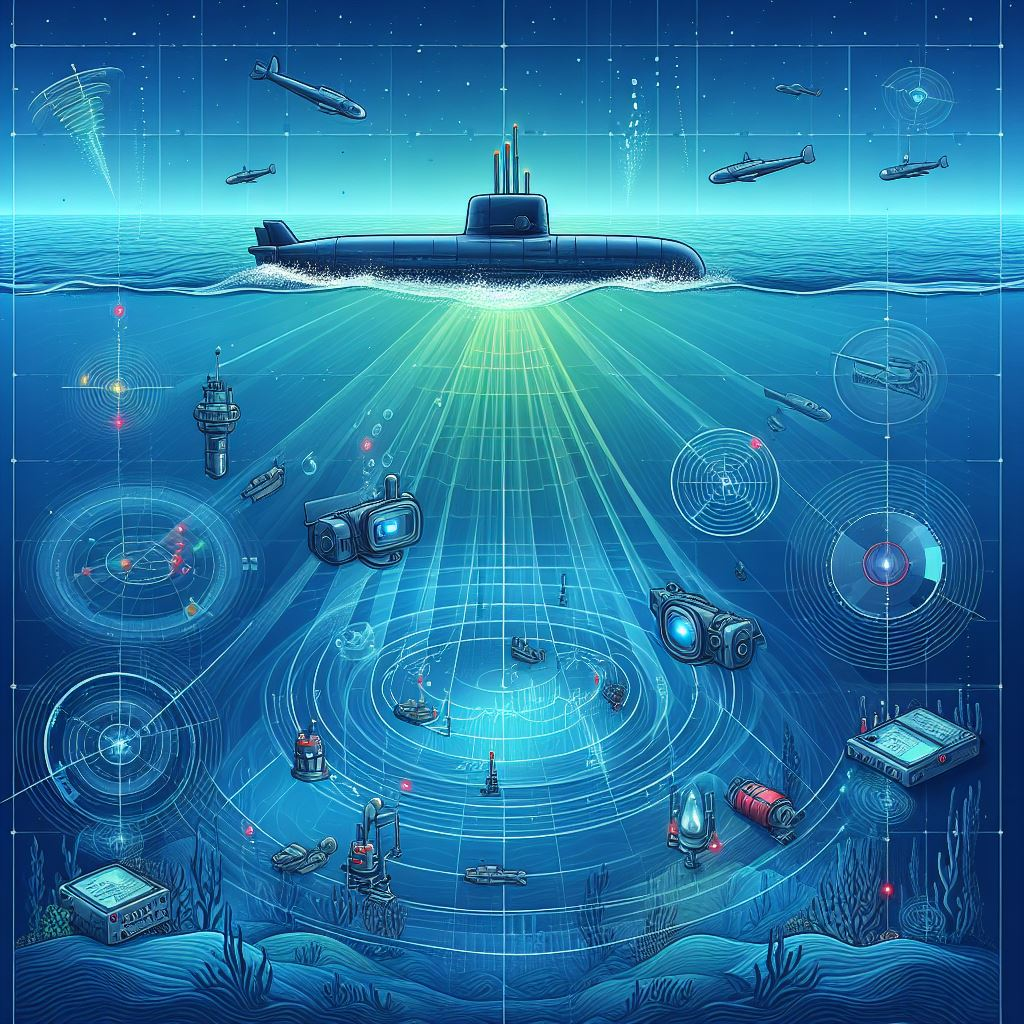
\includegraphics[width = 0.4\textwidth]{senarios.jpg}
    \caption{示例图}
    \label{fig:1_scene}
\end{figure}

在研究中\cite{RN35,RN33,RN34},示例段落。

丙辰中秋,欢饮达旦,大醉,作此篇,兼怀子由。(序)明月几时有?把酒问青天。不知天上宫阙,今夕是何年。

列表示例:
\begin{enumerate}[(1)]
    \setlength{\itemsep}{0.1em}
    \item 我欲乘风归去,又恐琼楼玉宇,高处不胜寒。起舞弄清影,何似在人间?转朱阁,低绮户,照无眠。
    \item 不应有恨,何事长向别时圆?人有悲欢离合,月有阴晴圆缺,此事古难全。
    \item 但愿人长久,千里共婵娟。
\end{enumerate}

他们具有不同的性能表现,如\cref{tab:1_1_comparison}所示。

\begin{table}[!h]
    \centering
    \caption{方案比较}
    \label{tab:1_1_comparison}
    \tabfont
    \begin{tabularx}{\textwidth}{X p{0.38\textwidth}p{0.38\textwidth}}
        \toprule
        {\heiti 类别} & {\heiti A类}        & {\heiti B类}          \\
        \midrule
        信号 & LFM、PMCW等。表格内超长文本内容示例。 & MFSK、OFDM等。表格内超长文本内容示例。 \\
        应用 & 感知、探测     & 信息传输       \\
        \bottomrule
    \end{tabularx}
\end{table}

\begin{table}[!hbt]
    \centering
    \caption{窄表}
    \label{tab:6_3}
    \tabfont
    \begin{tabular}{ccccc}
        \toprule
        {\heiti 方案}   & {\heiti AAA}             & {\heiti BBB}   & {\heiti CCC} & {\heiti DDD}                 \\
        \midrule
        参数1 & 1234            & $J$    & $J$  & $N \times J$            \\
        参数2 & 5678            & $J$    & $J$  & $N \times J$            \\
        \bottomrule
    \end{tabular}
\end{table}

\subsection{二级标题}
当声音在水中传播时,水声的速度公式可以表示为
\begin{equation}
    c = \frac {1} {\sqrt {\rho\beta}}.
    \label{eqn:1}
\end{equation}

公式交叉引用示例:如\cref{eqn:1}所示。

\subsubsection{三级标题}
暂时没设计4级标题。

\subsection{因此}

Conclusion goes here \dots

\

\printbibliography[heading=bibliography,title=参考文献]
\clearpage  % 换一页

\section{\textbf{项目的研究内容、研究目标,以及拟解决的关键科学问题}(此部分为重点阐述内容);}
\subsection{二级标题}
示例文字。

\subsubsection{三级标题}
示例文字。

\subsection{二级标题}
示例文字。

\subsubsection{三级标题}
示例文字。


\section{\textbf{拟采取的研究方案及可行性分析}(包括研究方法、技术路线、实验手段、关键技术等说明);}\
% 由于section风格定义为runin格式,section尾部的反斜杠为了换行,如果section紧接subsection可不用反斜杠

示例文字。

\section{\textbf{本项目的特色与创新之处;}}\

示例文字。
\section{\textbf{年度研究计划及预期研究结果}(包括拟组织的重要学术交流活动、国际合作与交流计划等)。}\

示例文字。

\part{\textbf{研究基础与工作条件}}
\section{\textbf{研究基础}(与本项目相关的研究工作积累和已取得的研究工作成绩);}\

示例文字。

\section{\textbf{工作条件}(包括已具备的实验条件,尚缺少的实验条件和拟解决的途径,包括利用国家实验室、国家重点实验室和部门重点实验室等研究基地的计划与落实情况);}\

示例文字。

\section{\textbf{正在承担的与本项目相关的科研项目情况}(申请人正在承担的与本项目相关的科研项目情况,\hskip -8pt 包括国家自然科学基金的项目和国家其他科技计划项目,要注明项目的资助机构、项目类别、批准号、项目名称、\hskip -5pt 获资助金额、\hskip -5pt 起止年月、\hskip -5pt 与本项目的关系及负责的内容等);}\

示例文字。

\section{\textbf{完成国家自然科学基金项目情况}(对申请人负责的前一个已资助期满的科学基金项目(项目名称及批准号)完成情况、后续研究进展及与本申请项目的关系加以详细说明。\hskip -8pt 另附该项目的研究工作总结摘要(限500字)和相关成果详细目录)。}\
% 添加标点符号的宽度控制,与模板说明性文字行数保持一致

示例文字。

\part{\textbf{其他需要说明的情况}}
\section{申请人同年申请不同类型的国家自然科学基金项目情况(列明同年申请的其他项目的项目类型、项目名称信息,并说明与本项目之间的区别与联系;\hskip -8pt 已收到自然科学基金委不予受理或不予资助决定的,无需列出)。}\

示例文字。

\section{具有高级专业技术职务(职称)的申请人是否存在同年申请或者参与申请国家自然科学基金项目的单位不一致的情况;\hskip -8pt 如存在上述情况,列明所涉及人员的姓名,申请或参与申请的其他项目的项目类型、\hskip -3pt 项目名称、\hskip -3pt 单位名称、\hskip -3pt 上述人员在该项目中是申请人还是参与者,并说明单位不一致原因。}\
% 添加标点符号的宽度控制,与模板说明性文字行数保持一致

示例文字。

\section{具有高级专业技术职务(职称)的申请人是否存在与正在承担的国家自然科学基金项目的单位不一致的情况;如存在上述情况,列明所涉及人员的姓名,正在承担项目的批准号、项目类型、项目名称、单位名称、起止年月,并说明单位不一致原因。}\

示例文字。

\section{同年以不同专业技术职务(职称)申请或参与申请科学基金项目的情况(应详细说明原因)。}\
% 新的模板新增项。

示例文字。

\section{其他。}\

示例文字。


\end{document}
